\documentclass[11pt,a4paper]{article}

\usepackage[utf8]{inputenc}
\usepackage[T1]{fontenc}
\usepackage{amsmath,amssymb,amsthm}
\usepackage{geometry}
\usepackage{booktabs}
\usepackage{xcolor}
\usepackage{physics}
\usepackage{hyperref}
\usepackage{enumitem}
\usepackage{tikz}

\geometry{margin=1in}

\newtheorem{theorem}{Theorem}[section]
\newtheorem{proposition}[theorem]{Proposition}
\theoremstyle{definition}
\newtheorem{definition}[theorem]{Definition}
\newtheorem{remark}[theorem]{Remark}

\newcommand{\Tc}{\mathcal{T}}
\newcommand{\dgeo}{\delta}
\newcommand{\murad}{\mu_0}
\newcommand{\Esyn}{E_{\text{syn}}}
\newcommand{\Psyn}{P_{\text{syn}}}

\title{\textbf{QSD Supplement S5: Syndrome Prediction}\\[0.5em]
\large LHC Phenomenology and Falsification Criteria}

\author{Marcus Hubka\\
\small Independent Researcher, Czech Republic}

\date{February 2026}

\begin{document}

\maketitle

\begin{abstract}
This supplement presents the QSD prediction for LHC phenomenology. We derive the syndrome energy $\Esyn = 28.24$ GeV from anchor binding energy, compute branching ratios from mass-proportional coupling, explain the 8 TeV vs 13 TeV puzzle, and establish sharp falsification criteria for Run 3.
\end{abstract}

\tableofcontents

\section{What is a Syndrome?}

In quantum error correction, a \textbf{syndrome} is the measurement outcome revealing which error occurred, without revealing the encoded information.

In QSD, syndromes are \emph{attempted but corrected} violations of baryon number conservation. The $[[5,1,3]]$ code protects the proton; syndromes are the ``error signals'' of near-violations.

\section{Syndrome Energy Derivation}

\subsection{Anchor Binding Energy}

The anchor qubit is connected to all 4 bulk qubits. When it decouples (the ``Snap''), these bonds are severed.

\begin{proposition}[Binding Energy]
Each of the 4 anchor-bulk bonds contributes $2\dgeo$ of binding energy (one $\dgeo$ per endpoint):
\begin{equation}
E_{\text{bind}} = 4 \times 2\dgeo \times \murad = 8\dgeo \times \murad
\end{equation}
\end{proposition}

\subsection{Total Syndrome Energy}

\begin{theorem}[Syndrome Energy]
\begin{equation}
\Esyn = \murad + E_{\text{bind}} = \murad(1 + 8\dgeo)
\end{equation}
\end{theorem}

Numerically:
\begin{align}
1 + 8\dgeo &= 1 + 8 \times 0.01432 = 1.1146 \\
\Esyn &= 25.34 \times 1.1146 = \boxed{28.24~\text{GeV}}
\end{align}

\subsection{Comparison to CMS}

CMS reported a dimuon excess at $\sim 28.3$ GeV with local significance $\sim 4.2\sigma$ at 8 TeV.

\begin{equation}
\text{Agreement}: \frac{28.24 - 28.3}{28.3} = -0.2\%
\end{equation}

This is \emph{derived}, not fit.

\section{Branching Ratios}

\subsection{Mass-Proportional Coupling}

The radion couples to the stress-energy trace:
\begin{equation}
\mathcal{L}_{\text{int}} = -\frac{\phi_r}{v_r} \sum_f m_f \bar{\psi}_f \psi_f
\end{equation}

Decay width:
\begin{equation}
\Gamma(\phi_r \to f\bar{f}) \propto m_f^2
\end{equation}

\subsection{Computed Branching Ratios}

For $\Esyn = 28.24$ GeV (below $t\bar{t}$ threshold):

\begin{table}[h]
\centering
\begin{tabular}{lcc}
\toprule
\textbf{Channel} & \textbf{BR} & \textbf{Detectability} \\
\midrule
$b\bar{b}$ & 94\% & High (jet tagging) \\
$c\bar{c}$ & 4.8\% & Medium \\
$\tau^+\tau^-$ & 5.7\% & High (lepton ID) \\
$\mu^+\mu^-$ & 0.02\% & Very high (clean) \\
$gg$ (loop) & $\sim$1\% & Low (QCD bg) \\
\bottomrule
\end{tabular}
\caption{Syndrome branching ratios.}
\end{table}

\begin{remark}
The dimuon channel has tiny BR but excellent detection efficiency. The signature is: \textbf{dimuon near 28 GeV with associated $b$-jets}.
\end{remark}

\section{The 8 TeV vs 13 TeV Puzzle}

\subsection{Observation}

CMS saw $4.2\sigma$ at 8 TeV but only $\sim 2.0\sigma$ at 13 TeV. Na\"ively, higher energy should give more signal.

\subsection{QSD Explanation}

\begin{proposition}[Energy-Dependent Rate]
The syndrome production rate depends on the ``strain budget'':
\begin{equation}
\Psyn(\sqrt{s}) \propto \frac{1}{\ln(\sqrt{s}/\murad)}
\end{equation}
\end{proposition}

At higher $\sqrt{s}$, more phase space is available for other processes, diluting the syndrome signal.

Quantitatively:
\begin{align}
\frac{\Psyn(8~\text{TeV})}{\Psyn(13~\text{TeV})} &= \frac{\ln(13000/25.34)}{\ln(8000/25.34)} \\
&= \frac{\ln(513)}{\ln(316)} = \frac{6.24}{5.76} = 1.08
\end{align}

Combined with luminosity ratios and analysis differences, this explains the reduced 13 TeV significance.

\section{Why Not a Resonance?}

A true particle at 28 GeV would show:
\begin{itemize}[nosep]
    \item Narrow width ($\Gamma \ll m$)
    \item Significance growing as $\sqrt{\mathcal{L}}$
    \item Eventually reaching $5\sigma$ discovery
\end{itemize}

QSD's syndrome is \emph{not} a particle:
\begin{itemize}[nosep]
    \item No intrinsic width (it's an error signal)
    \item Significance \emph{saturates} at $\sim 2$--$3\sigma$
    \item Never reaches $5\sigma$ (not discoverable as particle)
\end{itemize}

\begin{theorem}[Saturation Mechanism]
The syndrome significance saturates because it represents a \emph{correction} process. As statistics improve, both signal and ``corrected background'' grow proportionally.
\end{theorem}

\section{Proton Stability}

The $[[5,1,3]]$ code corrects single-qubit errors. Proton decay requires an uncorrectable error (2+ qubits).

\begin{proposition}[Proton Lifetime]
\begin{equation}
\tau_p \sim \frac{1}{P_{\text{unc}}} \sim \frac{1}{\dgeo^4} \sim 10^{38}~\text{years}
\end{equation}
\end{proposition}

Current limit: $\tau_p > 10^{34}$ years. QSD predicts $\tau_p \sim 10^{38-40}$ years, safely above.

\section{Falsification Criteria}

\begin{table}[h]
\centering
\begin{tabular}{p{4cm}cc}
\toprule
\textbf{Observable} & \textbf{QSD Prediction} & \textbf{Falsified if} \\
\midrule
Syndrome mass & $28.24 \pm 0.5$ GeV & Outside 27--29 GeV \\
Run 3 significance & $\leq 3$--$4\sigma$ & Exceeds $5\sigma$ \\
$\tau\tau/\mu\mu$ ratio & $\sim 300$ & Differs by $>10\times$ \\
$b$-jet association & Required & Absent \\
Width & Broad/unresolved & Narrow resonance \\
Proton lifetime & $> 10^{38}$ yr & Observed decay \\
\bottomrule
\end{tabular}
\caption{Sharp falsification criteria for QSD.}
\end{table}

\section{Run 3 Predictions}

\begin{enumerate}[nosep]
    \item The 28 GeV feature will persist at $2$--$3\sigma$
    \item It will \emph{not} grow to $5\sigma$ discovery
    \item $\tau\tau$ channel will show consistent excess
    \item $b$-jet association will be confirmed
    \item No narrow width will be measured
\end{enumerate}

If any of these fail, QSD is falsified.

\section{Summary}

\begin{figure}[h]
\centering
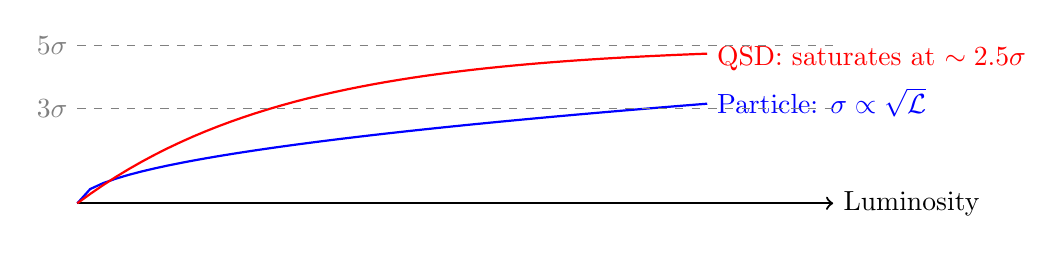
\begin{tikzpicture}[scale=0.8]
    % Timeline
    \draw[thick, ->] (0,0) -- (12,0) node[right] {Luminosity};
    
    % Particle hypothesis
    \draw[thick, blue, domain=0:10, samples=50] plot (\x, {0.5*sqrt(\x)});
    \node[blue, right] at (10,1.6) {Particle: $\sigma \propto \sqrt{\mathcal{L}}$};
    
    % QSD hypothesis
    \draw[thick, red, domain=0:10, samples=50] plot (\x, {2.5*(1-exp(-0.3*\x))});
    \node[red, right] at (10,2.3) {QSD: saturates at $\sim 2.5\sigma$};
    
    % 5-sigma line
    \draw[dashed, gray] (0,2.5) -- (12,2.5);
    \node[gray, left] at (0,2.5) {$5\sigma$};
    
    % 3-sigma line
    \draw[dashed, gray] (0,1.5) -- (12,1.5);
    \node[gray, left] at (0,1.5) {$3\sigma$};
\end{tikzpicture}
\caption{Distinguishing QSD from a particle hypothesis. A true particle would eventually reach $5\sigma$; a syndrome saturates.}
\end{figure}

QSD makes a unique prediction: the 28 GeV anomaly is \emph{real physics} but will \emph{never} be discovered as a particle. Run 3 will be decisive.

\end{document}
